%!TeX root=../tese.tex
%("dica" para o editor de texto: este arquivo é parte de um documento maior)
% para saber mais: https://tex.stackexchange.com/q/78101/183146

% Os capítulos de compõem a dissertação/tese, com numeração normal, podem
% ser inseridos diretamente aqui ou "puxados" de outros arquivos.
% Em alguns (raros) casos, pode ser interessante usar \include ao
% invés de \input: https://tex.stackexchange.com/a/32058/183146

\chapter{Introdução}
\label{chap:introducao}

Desde a pré-história, o ser humano tem a experiência de contar. Naquela época, o homem contava pequenas quantidades, 
como quantas pessoas tinham em seu bando ou quanto de alimento ele deveria coletar para sobreviver. Com o passar do 
tempo, o sistema numérico foi inventado para que pudéssemos trabalhar com valores cada vez maiores. 

\vspace{4mm}
\begin{figure}
  \centering
  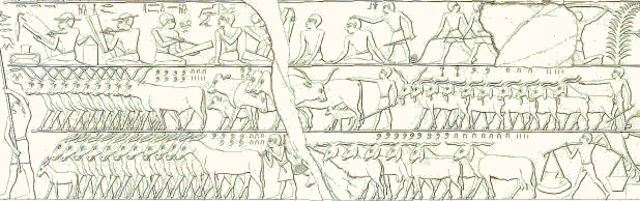
\includegraphics[width=\linewidth]{figuras/ancient_counting.png}
\end{figure} 
\vspace{2mm}

Quando pensávamos que contar não pudesse ficar mais difícil, os computadores surgem, abrindo novas discussões sobre a 
contagem. Entre elas, estavam como armazenar números em uma máquina, como fazer contas nesses aparelhos e até quanto 
poderíamos contar com a ajuda deles. E poucas décadas após essa invenção, a Internet é criada. 

Passamos, portanto, a ficar interessados em monitorar essa rede de computadores e para isso, tínhamos que descobrir 
quantas máquinas diferentes estavam acessando essa rede ou quem eram os aparelhos responsáveis pelo maior fluxo de dados. 
O principal desafio que surgiu nesse contexto, foi o alto volume de dados que precisavam ser processados em tempo real. 
E armazenar todos os dados localmente para em seguida, analisá-los deixou de ser viável devido à lentidão desse processo 
e ao elevado consumo de memória.

Estruturas de dados e algoritmos probabilísticos são uma forma de tentar contornar essa grande quantidade de informação. 
A ideia central é sacrificar a exatidão da resposta com o objetivo de consumir menos memória e tempo de processamento. 
Problemas que podem se beneficiar com soluções probabilísticas são, por exemplo, monitorar quantos usuários diferentes 
acessaram um site em um dado dia, contar quantas palavras distintas foram pesquisadas na última hora em uma plataforma 
de varejo ou armazenar quantas visualizações distintas um artigo teve. 

Uma característica comum desses problemas é que muitas vezes, suas respostas são métricas a serem utilizadas por outros 
sistemas com o intuito de se identificar falhas ou pontos de melhoria. No caso do monitoramento de quantas pessoas 
visitaram uma página web, uma forte queda nas visualizações pode ser um indício que um serviço esteja fora do ar. Nesse 
sentido, essas métricas não precisam ter necessariamente uma precisão de $100\%$, podendo apresentar um pequeno erro 
desde que sejam rapidademente computadas e leves de se armazenarem.

Por volta da década de~1970, Robert Morris tentou contar eventos cujo número de ocorrências não cabia na memória dos 
computadores da época~\citep{morris:78}. O \hyperref[chap:morris:algorithm]{algoritmo} proposto por ele serviu de 
inspiração para que outros autores conseguissem resolver problemas mais desafiadores, como a contagem distinta 
aproximada, cujo objetivo é estimar a quantidade de elementos distintos em um fluxo de dados. 

Alguns anos após Morris publicar o trabalho dele, a \hyperref[sec:flajolet-martin:algorithm]{$\pcounting$}, o primeiro 
algoritmo probabilístico que resolvia a contagem distinta aproximada, foi criada~\citep{flajolet:martin:85}. E a partir 
desse algoritmo, as soluções foram passando por melhorias, das quais podemos destacar a redução do consumo de memória, 
aumento da precisão e até mesmo o desenvolvimento de técnicas de demonstração que simplificavam o entendimento da razão 
desses algoritmos funcionarem.

Pouco tempo depois, as \hyperref[lab:chapter:04:01]{\asampling}, algoritmo que corrigia limitações da solução anterior, 
foram desenvolvidas~\citep{adptive:sampling:90}. Após uma década, a estrutura de dados 
\hyperref[sec:loglog:algorithm]{$\LOG$} é concebida, apresentando uma grande redução no consumo de 
memória~\citep{loglog:03}. E logo em seguida, o \hyperref[sec:loglog:hyperloglog]{$\HLOG$}, versão aperfeiçoada do 
$\LOG$, veio a público e se tornou uma das estruturas mais utilizadas para se resolver o problema da contagem distinta 
aproximada~\citep{hyperloglog:07}. Este texto, portanto, tem o objetivo de passar por essas soluções e apresentar 
comentários pertinentes de cada uma.

\vspace{2mm}
\begin{figure}
  \centering
  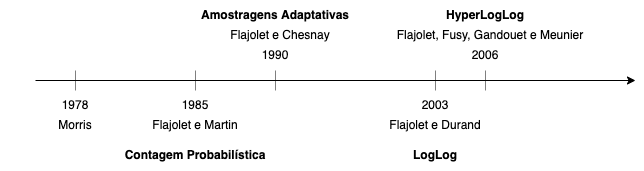
\includegraphics[width=\linewidth]{figuras/count_distinct_timeline.png}
\end{figure}  

\newpage
\section{Probabilidade}

Neste texto, serão discutidas soluções probabilísticas de problemas relacionados à contagem. Para entendê-las, alguns
conceitos relacionados à Estatística precisam estar claros.

\section{Variância}
\label{ap:variance}

Seja $X$ uma variável aleatória. Então,

\[ \mathbb{V}[X] = \mathbb{E}[X^2] - \mathbb{E}[X]^2\]

\section{Desigualdade de Markov}
\label{ap:markov}

Sejam $X$ uma variável aleatória e $\alpha > 0$ um número real. Então,

\[ \mathbb{P}(X \geq \alpha) \leq \frac{\mathbb{E}[X]}{\alpha^2}\]


\section{Desigualdade de Chebyshev}
\label{ap:chebyshev}

Seja $X$ uma variável aleatória com valor esperado $\mu$ finito e variância $\sigma^2$ finita e diferente de zero. 
Assim, para todo número real $k > 0$, 

\[ \mathbb{P}(| X - \mu| \geq k\sigma) \leq \frac{1}{k^2}\]

Outro modo de se escrever a desigualdade acima é 

\[ \mathbb{P}(| X - \mu| \geq k) \leq \frac{\sigma^2}{k^2} \]

\section{Transformação de Mellin}
\label{ap:mellin}

A transformação de Mellin para uma função \textit{real} $f(x)$ definida para $x \in \mathbb{R}$ e $x \geq 0$ é uma função 
\textit{complexa} $f^{*}(x)$ tal que:

\[ f^{*}(s) := M\big[f(x); s\big] = \int_{0}^{\infty} f(x)^{s-1} dx \ .\]
\par

\chapter{Contagem aproximada}
\label{chap:morris}


\section{O Problema}

O problema de contagem aproximada consiste em contar um grande número de eventos usando pouca memória.  
Esse problema foi abordado pela primeira vez por Robert  Morris (Morris, 1978). 
Neste artigo, o autor descreve a tentativa de se contar eventos cujas frequências podiam chegar até 130.000, mas só usando contadores de 8 bits.

Um registrador de n bits pode guardar valores até $2^n-1$. Dessa forma, em uma máquina que possui registradores de 8 bits, pode-se contar até 255.
Assim, o autor não conseguia manter as frequências exatas dos eventos devido à limitação de máquina. 
Contudo, ele podia armazenar contagens aproximadas.


\section{Ideias para solução}

Para se manter um contador exato até $n$, precisa-se de $O(\log n)$ bits. Para se conseguir contar até $n$ usando menos bits, 
deve-se abrir mão da exatidão da contagem. 

Uma das primeiras ideias é manter no contador o valor de $\log_2 n$ e assim, utilizar $O(\log \log n)$ bits de memória. 
A estimativa da contagem seria $2^x$, em que, $x$ é o valor armazenado no contador.

Outra ideia é como deve ser feita o incremento desse contador. 
A solução proposta por Morris é aumentar o contador com base em um método probabilístico, como pode ser visto no Programa \ref{prog:morris}. 


\section{Pseudocódigo}

\begin{programruledcaption}{Contagem aproximada: algoritmo de Morris\label{prog:morris}}
  \begin{lstlisting}[
    language={[brazilian]pseudocode},
    style=pseudocode,
    style=wider,
    functions={},
    specialidentifiers={},
  ]
      funcao Morris(M)  // Estima o tamanho de um conjunto de dados M
        X := 0  // Inicia o contador que guarda o logarítmo na base 2 do tamanho do conjunto M
        para cada dado do conjunto M faça
          para i de 0 até X faça
            jogue uma moeda 
          fim

          se todas as jogadas forem cara faça
            X := X + 1
          fim
        fim
      devolva $2^X - 1$
      fim
  \end{lstlisting}
\end{programruledcaption}

\section{Erro cometido}

Escrever a prova do algorimo \dots

\par

\newcommand{\bitmap}{\text{BITMAP}}
\newcommand{\pcounting}{\textit{probabilistic counting}}

\chapter{Contagem distinta aproximada: Flajolet-Martin (1985)}
\label{lab:flajolet-martin}

\section{O Problema}

\begin{quote}
  \textbf{Contagem Distinta:} Dado um conjunto $\Mbb$, \textbf{encontrar} quantos elementos \textit{distintos}
  $\Mbb$ possui.
\end{quote}

Uma solução para a \textbf{contagem distinta} é inserir cada elemento de $\Mbb$ em uma tabela hash. 
E assim, a quantidade de itens distintos nesse conjunto será o número de elementos nessa tabela.

Note que esse algoritmo consome $\Omega(n)$ de memória, uma vez que, deve-se armazenar cada elemento 
\textbf{pelo menos uma vez} para que seja possível verificar se um item está no conjunto.

Este consumo linear de espaço pode ser um problema quando a quantidade de elementos que precisam ser armazenados é muito 
grande. E podem existir aplicações nas quais é necessário manter \textbf{várias} dessas estruturas, como no caso do 
\textit{Redis}, em que se deseja encontrar quantos usuários distintos visualizararm um publicação ~\citep{Redis}. E para 
essas situações, é interessante que o consumo de memória seja muito menor que a quantidade de elementos distintos. 
Portanto, deve-se abandonar a exatidão da contagem dos elementos distintos para que se possa diminuir o consumo de 
espaço.

\begin{quote}
  \textbf{Contagem Distinta Aproximada:} dado um conjunto $\Mbb$, \textbf{estimar} o número de elementos 
  \textit{distintos} nesse conjunto.
\end{quote}

Uma das primeiras soluções para a \textbf{contagem distinta aproximada} foi apresentada por \textit{Philippe Flajolet} e 
\textit{Nigel Martin} no artigo ~\citep{flajolet:martin:85}.
A motivação para o desenvolvimento desse algoritmo foi a otimização de pesquisas em bancos de dados relacionais.
E a identificação do número de elementos distintos em uma coluna era a principal dificuldade nesse processo.

\section{Algoritmo de Flajolet-Martin}
\label{sec:flajolet-martin:algorithm}

O \textbf{algoritmo de Flajolet-Martin} utiliza uma função de hash $h$ que mapeia uniformemente cada elemento do 
conjunto $\Mbb$ para um número inteiro entre $0$ e $2^L-1$, em que $L$ é a quantidade necessária de bits para 
mapear todas as entradas de $\Mbb$ (na prática, este valor é $32$ ou $64$). Assim, para cada $x_i \in \Mbb$, 
será calculado um inteiro $y_i \coloneqq h(x_i)$. Note que $y_i$ pode ser visto como uma palavra binária aleatória de 
$L$ bits em que cada bit é gerado independentemente com probabilidade $\frac{1}{2}$. E o algoritmo é baseado na 
frequência das aparições dos prefixos dessas palavras aleatórias.

Então, suponha que palavras binárias aleatórias de $L$ bits estejam sendo geradas. Espera-se que a cada \textbf{2} 
palavras, pelo menos uma comece com \textbf{1}. E que a cada \textbf{4} palavras, pelo menos uma deva ter o prefixo 
\textbf{01}. Assim, a cada $\mathbf{2^k}$ palavras, espera-se que pelo menos uma palavra comece com $\mathbf{0^{k-1}1}$. 
Por outro lado, caso o prefixo $0^{k-1}1$ apareça, o esperado é que $2^{k}$ items já devam ter sido gerados. 

Dessa forma, o algoritmo mantém a ocorrência dos prefixos de cada $\textit{hash}$ em um vetor $\bitmap[0 \twodots L-1]$, 
de modo que $\bitmap[i] = 1$, se e somente se, o prefixo $0^i1$ apareceu entre os \textit{hashes} dos elementos de 
$\Mbb$. 

Note que é necessário mapear cada prefixo para um inteiro entre $0$ e $L - 1$. E para isso, defini-se a função $\rho$ 
que recebe um inteiro e devolve a posição do 1 menos significativo deste inteiro. Então, para um \textit{hash} $y$, 
suponha que $\rho(y) = k$. Assim, o prefixo da representação binária de $y$ é $0^k1$, e $\bitmap[k] = 1$. Um caso 
especial para essa função é quando o \textit{hash} é zero. Nesta situação, $\rho(0) = L$.

Por fim, seja $R$ o menor índice tal que $\bitmap[R] = 0$. A estimativa para o número de elementos distintos de 
$\Mbb$ será $2^R/\phi$, em que, $\phi$ é um fator de correção que será discutido em 
\refeq{sec:flajolet-martin:analysis}.

Segue o pseudocódigo:
\begin{programruledcaption}{
Algoritmo de Flajolet-Martin 
\\ \textbf{Entrada:} conjunto $\Mbb$, função de hash $h$, tamanho $L$ do vetor $\bitmap$ 
\\ \textbf{Saída:} quantidade de elementos distintos de $\Mbb$
\label{prog:flajolet-martin}
}
  \begin{lstlisting}[
    language={[brazilian]pseudocode},
    style=pseudocode,
    style=wider,
    functions={},
    specialidentifiers={},
  ]
      funcao FlajoletMartin($\Mbb$, h, L)
        para i de 0 até L \kw{faça}:
          $\bitmap[i]$ := 0
        fim
        para x $\in$ $\Mbb$ \kw{faça}:
          y := h(x)
          $\bitmap[\rho(y)]$ := 1
        fim
        R := 0
        enquanto $\bitmap[R]$ = 1 \kw{faça}:
          R := R + 1
        fim
        devolva $2^R/\phi$
      fim
  \end{lstlisting}
\end{programruledcaption}

\section{Análise do algoritmo}
\label{sec:flajolet-martin:analysis}

Suponha que a quantidade de elementos distintos de $\Mbb$ seja $n$. O valor esperado de $R$ definido na seção 
\refeq{sec:flajolet-martin:algorithm} é aproximadamente $\log_2(\phi n)$, em que $\phi = 0.77351\dots$ e o desvio padrão 
de $R$ é em torno de $1.12$. Essa seção busca mostrar as etapas da análise do Algoritmo~\ref{prog:flajolet-martin} feita 
por Flajolet e Martin. Os detalhes da prova podem ser vistos em ~\citep{flajolet:martin:85}.

O primeiro passo é entender que $R$ é uma estimativa para $\lfloor \log_2(n) \rfloor$. Pelo padrão das aparições dos 
prefixos dos hashes dos elementos de $\Mbb$, espera-se que $\bitmap[0]$ seja acessado aproximadamente $\lfloor 
\frac{n}{2} \rfloor$ vezes, $\bitmap[1]$ aproximadamente $\lfloor \frac{n}{4} \rfloor$ vezes $\dots$ Agora, para 
$k = \lfloor \log_2(n) \rfloor$, $\bitmap[k]$ deve ser acessado em torno de $\lfloor \frac{n}{2^{k+1}} \rfloor = 0$ 
vezes. Assim, o menor índice $R$ tal que o valor de $\bitmap$ seja zero é aproximadamente $\lfloor \log_2(n) \rfloor$.

Então, defini-se a variável aleatória $R_n$ como sendo o valor da variável $R$ ao final da execução do Algoritmo 
\ref{prog:flajolet-martin} para uma entrada $\Mbb$ com $n$ elementos distintos. Dessa forma, o interesse principal 
da demonstração é encontrar fórmulas ou estimativas para:
\begin{itemize}
  \item $p_{n,k} = \mathbb{P}(R_n = k)$: probabilidade de uma saída de \ref{prog:flajolet-martin} ser igual a $k$
  \item $q_{n,k} = \mathbb{P}(R_n \geq k)$: probabilidade de uma saída de \ref{prog:flajolet-martin} 
  ser maior ou igual a $k$
  \item $\Ebb[R_n]$: valor esperado de $R_n$
  \item $\Vbb[R_n]$: variância de $R_n$
\end{itemize}

O primeiro teorema de ~\citep{flajolet:martin:85} mostra uma fórmula \textit{exata} e \textit{discreta} para $q_{n,k}$. 
A principal idea para encontrar essa fórmula é agrupar as palavras binárias por prefixos da forma $0^k1$. Assim, 
defini-se $E_k = \{ x  \ | \ \rho(x) = k \}$, ou seja, $E_k$ é o conjunto de todas as palavras aleatórias com prefixos
iguais a $0^k1$. Da mesma forma, defini-se $K_k = \{ x \ | \ \rho(x) \geq k \}$. Em seguida, as diferentes entradas 
$\Mbb$ com $n$ elementos distintos são representadas por um polinômio:
\[ P_k^{(n)} = (E_0 + E_1 + \twodots + E_{k-1} + K_k)^n .\]

O próximo passo é tentar expandir esse polinômio usando \textit{inclusão e exclusão}, e associar uma medida 
probabilidade para $E_0, E_1, \twodots, E_{k-1}, K_k$. E a prova deste teorema termina encontrando uma relação entre 
$q_{n,k}$ e esta expansão de polinômio.

Em seguida, o Teorema 2 apresenta aproximações de $q_{n,k}$ para diferentes intervalos de $k$. E a consequência deste 
teorema é a existência de uma distribuição limitante para a distribuição de probabilidade de $R_n$ conforme $n$ cresce. 
Dessa forma, obtém-se uma fórmula \textit{aproximada} e \textit{contínua} para $q_{n,k}$:
\[ q_{n,k} \approx \psi(\frac{n}{2^k}) \]

em que, $\psi(x) = \prod_{j \geq 0} (1 - e^{-x2^j})$.

Note que por definição, $p_{n,k} = q_{n,k} - q_{n,k+1}$. Assim, pode-se aproximar $p_{n,k}$:
\[ p_{n,k} \approx \psi(\frac{n}{2^k}) - \psi(\frac{n}{2^{k+1}}) \ . \]

O interesse passa a ser, portanto, estimar $\Ebb[R_n]$ a partir dessa fórmula aproximada de $p_{n,k}$, de maneira 
que 
\[ \Ebb[R_n] = \sum_{k \geq 1} k p_{n,k} \approx \sum_{k \geq 1} k \Big[ \psi \Big( \frac{n}{2^k} \Big) - \psi 
  \Big( \frac{n}{2^{k+1}} \Big) \Big] \ . \]

Desse modo, defini-se a função real $F(x)$ como sendo
\[ F(x) =  \sum_{k \geq 1} k \Big[ \psi \Big( \frac{n}{2^k} \Big) - \psi \Big( \frac{n}{2^{k+1}} \Big) \Big] \ . \]

E o Lema 1 do artigo, afirma que 
\[ \Ebb[R_n] = F(x) + O \Big( \frac{1}{n^{0.49}} \Big) \ , \]
ou seja, que o valor esperado de $R_n$ se aproxima de $F(x)$ conforme $n$ cresce.

Em seguida, o Lema 2 apresenta o resultado da \hyperref[ap:mellin]{transformada de Mellin} de $F(X)$. A principal razão 
para se calcular essa transformação é que se pode expressar a fórmula inversa da transformada de Mellin como uma 
expansão assintótica cujos termos são resíduos da transformada. Assim, o Teorema $3A$ utiliza os Lemas 1 e 2, e o 
Teorema dos Resíduos para afirmar que 
\[ \Ebb[R_n] = \lg (\phi n) + P(\lg n) + o(1) \ , \]
em que, $P(x)$ é a expansão assintótica de $F(x)$ e $\phi = 0.77351\dots$, concluindo a prova que 
$\Ebb[R_n] \approx \lg (\phi n)$.

A prova para a estimativa de $\Vbb[R_n]$ segue os mesmos passos da prova anterior. Pela definição de 
\hyperref[ap:variance]{variância}, precisa-se estimar $\Ebb[R_n ^ 2]$. Assim, 
\[ \mathbb{E[R_n ^2]} = \sum_{k=1} k^2 p_{n,k} \approx G(x) \ , \]
em que
\[ G(x) = \sum_{k=1} k^2 p_{n,k} \ . \]

Dessa forma, encontra-se a transformada de Mellin de $G(x)$ e se analisa a inversa desta transformação para estimar 
$\Ebb[R_n^2]$.

\section{Melhorando precisão do algoritmo}

Na seção anterior, foi visto que $\Ebb[R_n] \approx \lg(\phi n)$, em que $\phi \approx 0.77351$. Assim, se o valor 
do contador $R$ no final do Algoritmo \ref{prog:flajolet-martin} para uma entrada com $n$ elementos distintos for 
aproximadamente igual a $\lg(\phi n)$, então a saída desse algoritmo é aproximadamente $n$. A tabela \ref{tab:flajolet} 
mostra que, em alguns casos, a saída do programa é praticamente igual a $n$ quando $R_n \approx \lg(\phi n)$.

\begin{center}
  \def\arraystretch{2}%
  \begin{table}
    \begin{tabular}{ |p{1.5cm}||p{2.5cm}|  }
      \hline
      \multicolumn{1}{|p{1.5cm}|}{\centering $n$ } 
      & \multicolumn{1}{|p{2.5cm}|}{\centering $(1 \slash \phi) 2^{\lg(\phi n)}$ }  \\
      \hline
      \multicolumn{1}{|p{1.5cm}|}{\centering 50 } 
      & \multicolumn{1}{|p{2.5cm}|}{\centering 49.99 }  \\
      \hline
      \multicolumn{1}{|p{1.5cm}|}{\centering 500 } 
      & \multicolumn{1}{|p{2.5cm}|}{\centering 500.0 }  \\
      \hline
      \multicolumn{1}{|p{1.5cm}|}{\centering 5000 } 
      & \multicolumn{1}{|p{2.5cm}|}{\centering 4999.99 }  \\
      \hline
      \multicolumn{1}{|p{1.5cm}|}{\centering 50000 } 
      & \multicolumn{1}{|p{2.5cm}|}{\centering 50000.0 }  \\
      \hline
     \end{tabular}
     \caption{\label{tab:flajolet} Comparação entre $n$ e saída do Algoritmo \ref{prog:flajolet-martin} para 
     $R_n = \lg(\phi n)$.}
  \end{table}
\end{center}

Contudo, $\Vbb[R_n] \approx\nolinebreak 1.12$ e consequentemente, o desvio padrão de $R_n$ é aproximadamente~$1$. 
Isto quer dizer que o valor de $R_n$ pode ser uma unidade maior ou menor que $\lg(\phi n)$, o que implica que a 
estimativa de $n$ possa ser duas vezes maior ou menor que $n$. Logo, o Algoritmo de Flajolet e Martin apresenta uma 
grande variabilidade.

Assim como foi visto na Seção \ref{sec:morris:plus}, pode-se diminuir a variância da estimativa fazendo $k$ iterações 
do Algoritmo \ref{prog:flajolet-martin}. Dessa forma, seria necessário manter $k$ vetores \bitmap, $k$ valores de $R$ e 
$k$ funções de hash $h$. Ao final de todas as $k$ iterações, seria calculado a média $\bar{R}$ dos valores de $R$, e a 
estimativa do número de elementos distintos seria $(1 \slash \phi) 2^{\bar{R}}$.

O pseudocódigo a seguir codifica essa idea:

\begin{programruledcaption}{
  Algoritmo de Flajolet-Martin+
  \\ \textbf{Entrada:} conjunto $\Mbb$, $k$ funções de hash, tamanho $L$ do vetor $\bitmap$ 
  \\ \textbf{Saída:} quantidade de elementos distintos de $\Mbb$
  \label{prog:flajolet-martin+}
  }
    \begin{lstlisting}[
      language={[brazilian]pseudocode},
      style=pseudocode,
      style=wider,
      functions={},
      specialidentifiers={},
    ]
        funcao FlajoletMartin($\Mbb$, k, h, L)
          para i de 0 até k \kw{faça}:
            para j de 0 até L \kw{faça}:
              $\bitmap_i[j]$ := 0
            fim
          fim
          para i de 0 até k \kw{faça}:
            para x $\in$ $\Mbb$ \kw{faça}:
              y := $h_i(x)$
              $\bitmap_i[\rho(y)]$ := 1
            fim
          fim
          para i de 0 até k \kw{faça}:
            $R_i$ := 0
          fim
          para i de 0 até k \kw{faça}:
            enquanto $\bitmap_i[R_i]$ = 1 \kw{faça}:
              $R_i$ := $R_i$ + 1
            fim
          fim
          $\bar{R}$ := 0
          para i de 0 até k \kw{faça}:
            $\bar{R}$ := $\bar{R} + R_i$ 
          fim
          $\bar{R}$ := $\bar{R} \slash k$
          devolva $2^{\bar{R}}/\phi$
        fim
    \end{lstlisting}
  \end{programruledcaption}

Seja $\bar{R_n}$ o valor da variável $\bar{R}$ ao final da execução do Algoritmo \ref{prog:flajolet-martin+} para uma
entrada com $n$ elementos distintos. De forma análoga aos resultados vistos na Seção \ref{sec:morris:plus}, pode-se
concluir que:
\[ \Ebb[\bar{R_n}] \approx \lg(\phi n)  \; \; \text{e}  \; \; \Vbb[\bar{R_n}] \approx \frac{1.12}{k} \ . \]


No entanto, o fato de se precisar de uma função de hash distinta para cada iteração torna a solução acima inviável, 
uma vez que, encontrar funções de hash que mapeiem na prática os elementos de um conjunto $\Mbb$ de maneira
uniforme não é uma tarefa simples. Para contornar esse problema, os autores propuseram o uso da 
\textit{média estocástica}.

Essa ideia consiste em dividr os elementos da entrada em $k$ lotes e usar parte da informação do hash para definir em 
qual lote um elemento deve ir. 
As linhas de $7$ até $11$ do pseudocódigo a seguir mostram como esta divisão é feita:
\begin{programruledcaption}{
  Algoritmo de Flajolet-Martin++
  \\ \textbf{Entrada:} conjunto $\Mbb$, funções de hash $h$, tamanho $L$ do vetor $\bitmap$, 
  quantidade $k$ de lotes
  \\ \textbf{Saída:} quantidade de elementos distintos de $\Mbb$
  \label{prog:flajolet-martin++}
  }
    \begin{lstlisting}[
      language={[brazilian]pseudocode},
      style=pseudocode,
      style=wider,
      functions={},
      specialidentifiers={},
    ]
        funcao FlajoletMartin($\Mbb$, k, h, L)
          para i de 0 até k \kw{faça}:
            para j de 0 até L \kw{faça}:
              $\bitmap_i[j]$ := 0
            fim
          fim
          para x $\in$ $\Mbb$ \kw{faça}:
            lote := $h(x) \mod k$
            y := $\lfloor h(x) / k \rfloor$
            $\bitmap^{<lote>}[\rho(y)]$ := 1
          fim
          para i de 0 até k \kw{faça}:
            $R_i$ := 0
          fim
          para i de 0 até k \kw{faça}:
            enquanto $\bitmap_i[R_i]$ = 1 \kw{faça}:
              $R_i$ := $R_i$ + 1
            fim
          fim
          $\bar{R}$ := 0
          para i de 0 até k \kw{faça}:
            $\bar{R}$ := $\bar{R} + R_i$ 
          fim
          $\bar{R}$ := $\bar{R} \slash k$
          devolva $k2^{\bar{R}}/\phi$
        fim
    \end{lstlisting}
  \end{programruledcaption}

Se a função de hash $h$ distribuir os $n$ elementos distintos do conjunto $\Mbb$ uniformemente entre os 
$k$ lotes, então espera-se que cada lote tenha aproximadament $\frac{n}{k}$ elementos. Dessa forma, 
$(1 / \phi)2^{\bar{R_n}}$ seria uma aproximação para $\frac{n}{k}$. É devido a este fato que a saída do Algoritmo~
\ref{prog:flajolet-martin++} é $\mathbf{k} (1 / \phi)2^{\bar{R_n}}$, pois este valor é uma estimativa para 
$\mathbf{k} \frac{n}{k} = n$.

Por fim, o erro relativo esperado do algoritmo \proc{ProbabilisticCounting++} é em torno de $0.78 / \sqrt{m}$. Isto quer 
dizer que para $m = 64$, o desvio esperado é em torno de $10\%$. Dessa forma, a escolha de $m$ depende das exigências do 
problema. Se precisarmos de uma precisão maior, escolheremos um valor de $m$  maior, mas teremos um algoritmo mais 
custoso em termos de tempo e espaço. Por outro lado, se a exigência é, por exemplo, decidir qual de dois conjuntos tem a 
menor quantidade de elementos distintos, podemos escolher um valor menor de $m$ para fazer essa comparação, mas teríamos 
um risco maior de escolher o conjunto errado.

\section{Limitações do algoritmo $\pcounting$}

Uma das principais razões para escolhermos algoritmos \textit{probabilísticos} ao invés de algoritmos \textit{exatos} é 
o \textbf{consumo de memória reduzido}. Por exemplo, para resolver o problema da contagem distinta de forma 
\textit{exata}, podemos manter uma tabela de hash e conforme os elementos forem processados, adicionar a esta tabela 
somente aqueles elementos que não apareceram ainda. Assim,  quantidade de elementos distintos processados será o tamanho 
da tabela. Suponha que cada hash seja um inteiro de 4 bytes (32 bits) e que existam um milhão de itens distintos 
percorridos. Para armazenar essa tabela, gastaríamos pelos menos 4 MB. Por outro lado, se usarmos o algoritmo 
$\pcounting$ para resolver esse problema, o consumo de memória seria proporcional ao valor $m$ e não dependeria da 
quantidade de itens distintos. Logo, se o vetor $\bitmap$ for um vetor de inteiros de 4 bytes de tamanho $m$, e 
$m$ for igual a 1024, então a memória consumida por esse algoritmo seria em torno de 4 KB, que é um consumo de espaço
\textbf{1000 vezes menor} que a solução exata.

O erro relativo esperado do $\pcounting$ para $m = 1024$ é em torno de $2{,}5\%$. Assim, para um conjunto de milhões de 
itens distintos, o erro seria em torno das dezenas ou centenas de milhares. Com esse tipo de desvio, teríamos como 
mensurar a ordem de grandeza do número de itens distintos de um conjunto com bastante confiança. Contudo, para utilizar
o $\pcounting$, o viés desse algoritmo deve ser entendido.

O \textbf{viés} de um estimador é a diferença entre seu valor esperado e o valor real do parâmetro estimado. Nesse sentido, a 
estimativa da quantidade de elementos em um conjunto devolvida pelo algoritmo de \proc{Morris} é \textit{não-viesada}, 
uma vez que, o Lema \ref{morris:expected_value} afirma que o valor esperado deste estimador é igual ao tamanho do 
conjunto estimado.

Na prova descrita em ~\citep{flajolet:martin:85}, o estimador de $\lg(n)$ é $R_n$, que representa o valor da variável 
$R$ ao final da execução de \proc{ProbabilisticCounting}, tendo como entrada um conjunto com $n$ elementos distintos. 
Vimos que o valor esperado de $R_n$ é aproximadamente $\lg(\phi n)$, que é diferente de $\lg(n)$. Portanto, $R_n$ é um 
estimador \textit{viesado} de $\lg(n)$. E analogamente, o estimador devolvido por \proc{ProbabilisticCounting++} também 
é \textit{viesado}.  

Então, além do erro padrão, existe também o viés do algoritmo $\pcounting$, cujo valor é $1 + 0{,}31/m$. Contudo, para 
valores de $m$ maiores que $32$, o viés se torna desprezíval se comparado ao erro padrão. Dessa forma, uma pessoa pode 
ser induzida a concluir que a escolha de $m$ é o único cuidado que ela deve tomar ao utilizar esse algoritmo. No 
entanto, ainda existe o problema de estimar \textit{baixas cardinalidades} com essa estrutura.

Suponha, portanto, que $m = 64$ e que o hash do único elemento de um conjunto $\Mbb$ comece com $1$. Logo, se passarmos 
$\Mbb$ para \proc{ProbabilisticCounting++}, existiria um vetor $\bitmap$ cuja primeira posição teria o valor $1$, e o 
restante dos vetores $\bitmap$ teriam todos valores zero. Assim, $\bar{R}$ será igual a $1/64$, e o estimador de $n$ 
terá o valor de $64 \ 2^{\frac{1}{64}}/\phi \approx 83.64$. Esta estimativa está muito distante do valor real, que é 
$n = 1$.

Em vista disso, um tratamento especial deve ser dado para situações em que a cardinalidade do número de elementos 
distintos de um conjunto for baixa. Poderíamos, por exemplo, manter os elementos percorridos em uma tabela de hash, e 
quando essa tabela atingisse um certo tamanho, passaríamos a usar a estratégia original do $\pcounting$, que é preencher
os vetores $\bitmap$.  
\par

\newcommand{\asampling}{\proc{Amostragens Adaptativas}}
\newcommand{\AS}{\proc{AdaptiveSampling}}

\chapter{Contagens por amostragens}

Este capítulo aborda uma outra solução para o problema da contagem distinta aproximada. O 
Capítulo~\ref{lab:flajolet-martin} apresentou o algoritmo da $\pcounting$, que estima o número de elementos distintos em 
um fluxo de dados com desvio padrão em torno de $0.78 / \sqrt{m}$. 

O algoritmo das $\asampling$ tem um desvio padrão de aproximadamente $1.20 / \sqrt{m}$~\citep{adptive:sampling:90}. 
As razões para estudarmos esse algoritmo mesmo que ele apresente um erro maior ficarão claras nas próximas seções.

\section{Algoritmo das $\asampling$}
\label{lab:chapter:04:01}

O algoritmo das $\asampling$ também se baseia em \hyperref[sec:flajolet-martin:pattern]{padrões de bits} dos hashes dos 
elementos examinados. Podemos dessa forma, considerar que os elementos que estamos contando são palavras binárias de 
tamanho infinito. 

Enquanto que no algoritmo da $\pcounting$, estávamos interessados na \textbf{aparição} de um elemento com 
prefixo da forma $0^*1$, no algoritmo das $\asampling$, queremos saber a \textbf{quantidade} de elementos com um certo 
prefixo $0^*$.

Nesse sentido, vamos manter um contador $\delta$ cujo valor inicialmente é zero, e uma lista que armazena elementos com 
prefixo $0^{\delta}$. Para cada elemento examinado, inserimos ele na lista se o prefixo dele for da forma $0^{\delta}$.
Quando essa lista tiver mais que $m$ elementos, incrementamos $\delta$ em 1 e passamos a manter 
somente elementos com prefixo $0^{\delta + 1}$.

Agora, suponha que em um dado momento do algoritmo, a lista tenha tamanho $l$ e estamos mantendo somente elementos com 
prefixos $0^{\delta}$. A probabilidade de um elemento ter um prefixo dessa forma é $1 / 2^{\delta}$, e consequentemente,
esperamos que a cada $2^{\delta}$ itens, pelo menos um item tenha um prefixo desse formato. Assim, se nossa lista tem
$l$ elementos com prefixo $0^{\delta}$, então devemos ter examinado pelo menos $2^{\delta} l$ itens, e este valor é 
justamente a estimativa para a quantidade de valores distintos.

O algoritmo $\AS$ recebe um fluxo $\Mbb$ com $n$ elementos distintos e um parâmetro $m$, que está relacionado com o 
consumo de memória do algoritmo e sua precisão. O algoritmo usa uma função de hash $h$ para associar de forma uniforme 
os elementos de~$\Mbb$ a inteiros de~$L$ bits, e quanto maior for este valor, menor será a quantidade de colisões. Por 
fim, o valor devolvido é um estimador~$\hat{n}$ para $n$ da forma $2^{\delta} l$, em que $l$ e $\delta$ indicam que 
estão sendo armazenados $l$ elementos cujos prefixos tem formato~$0^{\delta}$. 

\begin{codebox}
  \Procname{$\AS(\Mbb, m)$}
  \li $LIST \gets \emptyset$
  \li $\delta \gets 0$
  \li \For cada $x$ em $\Mbb$ 
  \li    \Do 
         \If $0^{\delta}$ é prefixo de $h(x)$ \textbf{e} $h(x) \not\in LIST$
  \li             \Then $LIST \gets LIST \cup \{ h(x) \}$
         \End
  \li    \While $|LIST| > m$                                   \label{li:as:while}
  \li    \Do
         $\delta \gets \delta + 1$
  \li    $TEMPLIST \gets \emptyset$
  \li    \For cada $y$ em $LIST$
  \li    \Do
            \If $0^{\delta}$ é prefixo de $h(y)$
  \li       \Then $TEMPLIST \gets TEMPLIST \cup \{ h(y) \}$
            \End
         \End
  \li    $LIST \gets TEMPLIST$
         \End 
      \End
  \li
  \Return $2^{\delta} |LIST|$   
  \End
\end{codebox}


\section{Vantagens das $\asampling$}
\label{lab:chapter:04:02}

Vamos simular um exemplo pequeno para ver o funcionamento do algortimo $\AS$. Assim, queremos estimar quantos elementos 
distintos o fluxo $\Mbb = \{ 36, 108, 41, 82, 71, 61, 5, 54, 10 \}$ possui. Vamos considerar que a função de hash~$h$ é
a identidade, ou seja, $h(x) = x$ para todo $x$ em $\Mbb$, e que $m = 3$. 

Inicialmente, a lista $LIST$ está vazia e $\delta = 0$. Na primeira iteração do algoritmo, temos que verificar se o 
prefixo da representação binária do elemento $36 = 001001_2$ é da forma $0^0$. Note que qualquer elemento passará nessa 
validação quando $\delta$ for zero, uma vez que, uma palavra binária precisar ter o prefixo $0^0$ significa que ela tem 
que começar com 0 zeros, ou seja, pode começar com 0 ou com 1. Dessa forma, podemos inserir o elemento $36$ na lista, de 
modo que $LIST = \{ 36 \}$. Na próxima iteração, temos que fazer a mesma verificação anterior, só que usando o item de 
valor 108. Novamente, como $\delta = 0$, podemos adicionar $108$ à lista. Analogamente, podemos incluir os elementos 
$41$ e $82$ em $LIST$. 

Contudo, na quarta iteração, entramos no \texttt{while} da linha~\ref{li:as:while}, já que $|LIST| = 4 > m = 3$. Por 
conta disso, incrementamos o valor de $\delta$ e devemos manter em $LIST$ somente aqueles valores cujos prefixos de suas 
representações binárias são da forma $0^{1}$. Vamos ver quais elementos estão em $LIST$:
\[ 
       LIST = \{ 36 = 001001_2, 108 = 0011011_2, 41 = 100101_2, 82 = 0100101_2 \} \  .        
\] 
Precisamos manter nessa lista, somente aqueles números com prefixos que começam com~0. Assim, temos que remover o valor 
41 de $LIST$. 

Continuando o exemplo, precisamos verificar se adicionaremos $71 = 1110001_2$ na lista. Agora, os elementos em $LIST$ 
precisam começar com zero, logo 71 não é inserido. A mesma situação ocorre para os valores $61 = 101111_2$ e 
$5 = 101_2$. Em seguida, podemos inserir $54 = 011011_2$ em $LIST$ e como novamente, $|LIST| = 4 > 3$, teremos que 
incrementar $\delta$ e filtrar os itens da lista. A lista atual é 
\[ \{ 36 = 001001_2, 108 = 0011011_2, 82 = 0100101_2, 54 = 011011_2 \} \ . \] 
Manteremos somentes os valores cujos prefixos binários se iniciam com dois zeros e portanto, 
\[ LIST = \{ 36 = 001001_2, 108 = 011011_2 \} \ . \]
Por fim, o valor $10 = 0101_2$ não é inserido na lista. E a estimativa para a quantidade de elementos distintos em 
$\Mbb$ é $2^{\delta} \times |LIST| = 2^2 \times 2 = 8$. Essa estimativa está cometendo um erro de um item, já que $\Mbb$
tem 9 itens distintos. 

O fato curioso desse exemplo acontece nas primeiras iterações, quando $\delta$ tem valor zero. Vimos que qualquer 
elemento de $\Mbb$ nessas primeiras iterações é inserido em $LIST$. Nessas situações, a estimativa do algoritmo é 
$2^{\delta} \times |LIST| = 2^{0} \times |LIST| = |LIST|$. Ou seja, para os primeiros $m$ itens distintos de $\Mbb$, a 
estimativa tem precisão de $100\%$. Isto é o principal diferencial do algoritmo das $\asampling$ para o algoritmo da 
$\pcounting$, que como foi visto em \hyperref[sec:fm:low_estimates]{Estimando valores pequenos com a $\pcounting$}, 
apresenta um erro muito grande quando queremos estimar cardinalidades baixas.

Outro fator importante de se destacar é que o estimador devolvido por $\AS$ é 
\textbf{não-viesado}~\citep{adptive:sampling:90}. Essa característica está relacionada com o fato do algoritmo das 
$\asampling$ poder estimar valores pequenos sem problemas.

\newpage
\section{Implementando $\asampling$}

Nesta seção apresentaremos a implementação do algoritmo das \proc{Amostragens} \proc{Adaptativas} e experimentos.

\begin{lstlisting}[style=mypython,caption=Implementação do algoritmo $\AS$,captionpos=b, label=as:code]
class AdaptiveSampling:
    def __init__(self, m=64, L=64):
        self.delta: int = 0
        self.m: int = m
        self.L: int = L
        self.LIST: Set[int] = set()
   
    def zeros_no_prefixo(self, x: int):
        return (x & -x).bit_length() - 1

    def adiciona(self, x: int):
        if x not in self.LIST and self.zeros_no_prefixo(x) >= self.delta:
            self.LIST.add(x)

        while len(self.LIST) > self.m:
            self.delta = self.delta + 1
            temp: Set[int] = set()

            for y in self.LIST:
                if self.zeros_no_prefixo(y) >= self.delta:
                    temp.add(y)

            self.LIST = temp

    def conta(self):
        return (1 << self.delta) * len(self.LIST)
\end{lstlisting}

Vamos comentar alguns aspectos do código do Programa~\ref{as:code} baseado no algoritmo~$\AS$. O primeiro detalhe de 
implementação desse programa é que a função de hash~$h$ é implicitamente a função identidade, uma vez que, estamos 
supondo que os elementos inseridos são inteiros gerados uniformemente. O próximo detalhe é a estrutura de dados 
utilizada para representar a lista $LIST$. Foi escolhido um \proc{Set} para representá-la, que é uma estrutura padrão do 
\proc{Python} que permite inserir elementos e verificar se um elemento está presente nela em tempo constante. Dessa 
forma, a complexidade do método~\texttt{adiciona} é $O(1)$ amortizado.

Por fim, falta esclarecer como foi codificada a verificação se um inteiro tem prefixo da forma $0^{\delta}$, ou em 
outras palavras, se a representação binária de um inteiro começa com pelo menos $\delta$ zeros. Lembremos dessa forma, 
da função $\rho$ definida na Seção~\ref{sec:flajolet-martin:algorithm}. Essa função recebe um inteiro $x$ e devolve a 
posição indexada a partir do zero do bit menos significativo de $x$. Assim, $\rho(12) = \rho(0011_2) = 2$ e 
$\rho(24) = \rho(00011_2) = 3$. Note que a saída da função $\rho$ corresponde também a quantidade de bits zeros no 
prefixo da representação binário de um inteiro. Podemos, portanto, aproveitar o método $p$ da classe 
\texttt{ProbabilisticCounting} para implementar o método \texttt{zeros\_no\_prefixo} e agora, para verificar se um 
inteiro~$x$ tem prefixo da forma $0^{\texttt{delta}}$, basta testar se \texttt{zeros\_no\_prefixo(x)} é maior ou igual a
\texttt{delta}.

A partir deste ponto, apresentaremos experimentos do algoritmo das \proc{Amostragens} \proc{Adaptativas}, que serão os 
mesmos realizados na Seção~\ref{sec:fm:experiments}, só que utilizando a estrutura apresentada nesse capítulo. Assim, o 
primeiro experimento que veremos é observar a evolução das estimativas devolvidas pela estrutura
~\texttt{AdaptiveSampling} conforme mais itens são inseridos nela. Portanto, nas simulações realizadas, inserirmos um 
milhão de inteiros de 64 bits distintos gerados uniformemente em estruturas com $m = 64$ e $m = 1024$. E o mesmo gerador 
de números pseudo-aleatórios dos experimentos do algoritmo da~$\pcounting$ foi utilizado, ou seja, os mesmos elementos 
foram aproveitados.

Os resultados do primeiro experimento podem ser observados na Figura~\ref{fig:as:experimento:01}. É possível perceber
que a estrutura com o parâmetro $m$ maior teve uma precisão melhor que a estrutura com $m$ menor ao longo de toda a 
simulação. 

\begin{figure}
  \centering
  \begin{subfigure}{.5\textwidth}
    \centering
    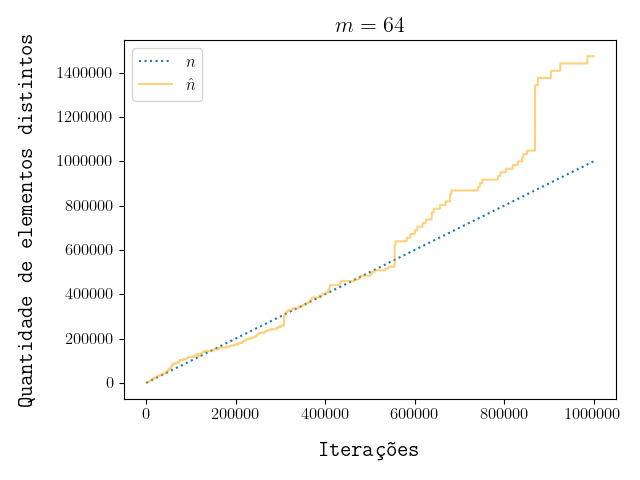
\includegraphics[width=\linewidth, height=4cm]{figuras/adaptive_sampling_full_64.png}
  \end{subfigure}%
  \begin{subfigure}{.5\textwidth}
    \centering
    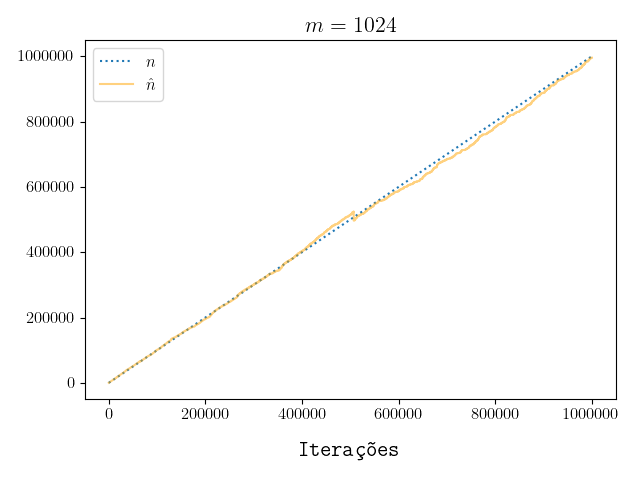
\includegraphics[width=\linewidth, height=4cm]{figuras/adaptive_sampling_full_1024.png}
  \end{subfigure}
  \caption{Primeiro experimento do algoritmo $\AS$. Foram inseridos em estruturas \texttt{AdaptiveSampling} com $m = 64$ 
  e $m = 1024$, um milhão de inteiros de 64 bits gerados uniformemente.}
  \label{fig:as:experimento:01}
\end{figure}


Os gráficos com a evolução do erro relativo do experimento anterior estão na Figura~\ref{fig:as:experimento:01:erro}.
O desvio padrão do algoritmo das $\asampling$ é $1.20/\sqrt{m}$. Portanto, para a estrutura com $m = 64$, o desvio 
padrão é de $15\%$. As estimativas devolvidas por essa estrutura ficaram entre dois desvios padrões na maior parte da 
simulação, apresentando um erro maior quando esta se aproximava do fim. Já a estrutura com $m = 1024$ tem desvio padrão 
de $3{,}75\%$, e a simulação dela teve valores que ficaram dentro de um desvio na maior parte das iterações.

\begin{figure}
  \centering
  \begin{subfigure}{.5\textwidth}
    \centering
    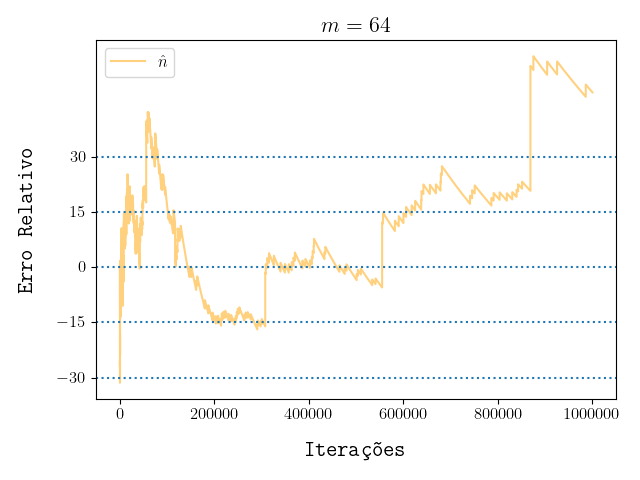
\includegraphics[width=\linewidth, height=4cm]{figuras/adaptive_sampling_erro_full_64.png}
  \end{subfigure}%
  \begin{subfigure}{.5\textwidth}
    \centering
    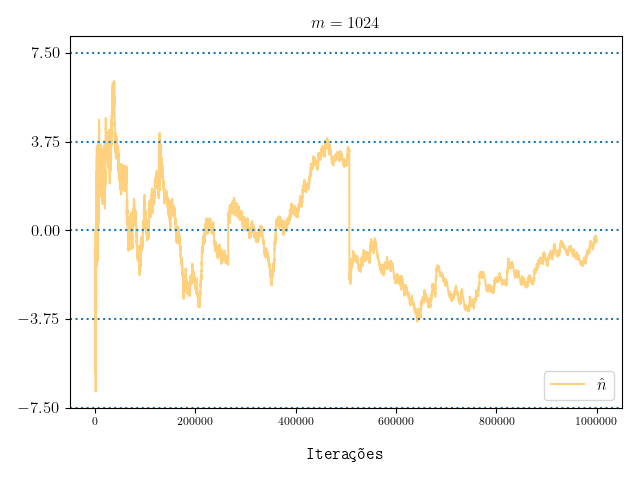
\includegraphics[width=\linewidth, height=4cm]{figuras/adaptive_sampling_erro_full_1024.png}
  \end{subfigure}
  \caption{Erro relativo do primeiro experimento do algoritmo $\AS$. Para $m = 64$, o erro ficou dentro de dois desvios
  padrões. Para $m = 1024$, a faixa de erro foi de um desvio padrão.}
  \label{fig:as:experimento:01:erro}
\end{figure}

Antes de passarmos para o segundo experimento, é interessante verificarmos se o que foi discutido na 
Seção~\ref{lab:chapter:04:02} pode ser observado nas simulações anteriores. Queremos, assim, averiguar se o algoritmo 
das~$\asampling$ funciona de fato para baixas cardinalidades. A Figura~\ref{fig:as:experimento:01:erro:first} tem
gráficos que destacam o erro relativo nas primeiras~256 iterações no caso da estrutura com $m = 64$ e nas primeiras~1024
iterações no caso da estrutura com $m = 1024$. Nos dois casos, podemos notar que o erro relativo nas primeiras~$m$ 
iterações é de fato zero e que o erro após essas iterações iniciais se manteve controlado, dentro da faixa de dois 
desvios padrões.

\begin{figure}
  \centering
  \begin{subfigure}{.5\textwidth}
    \centering
    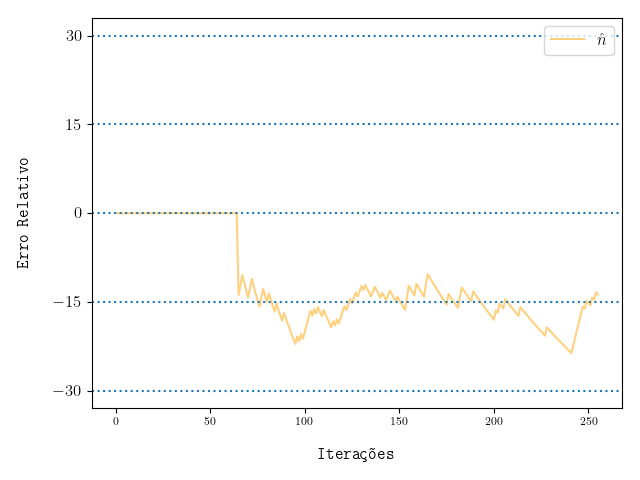
\includegraphics[width=\linewidth, height=4cm]{figuras/adaptive_sampling_erro_first_64.png}
  \end{subfigure}%
  \begin{subfigure}{.5\textwidth}
    \centering
    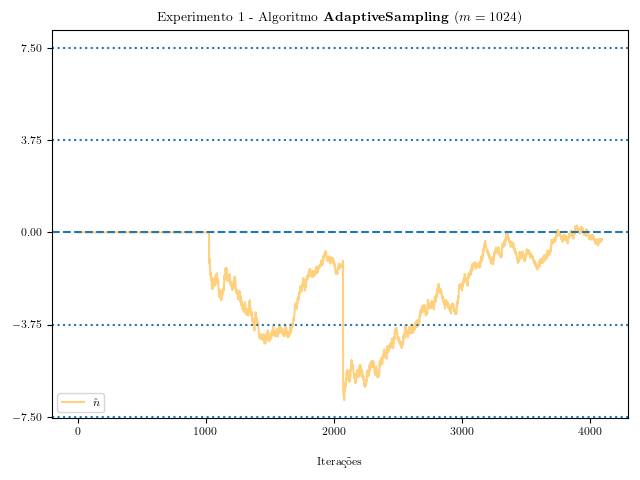
\includegraphics[width=\linewidth, height=4cm]{figuras/adaptive_sampling_erro_first_1024.png}
  \end{subfigure}
  \caption{Erro relativo nas primeiras iterações do experimento do algoritmo~$\AS$. Nas $m$ inserções iniciais,o erro 
  relativo do algoritmo é zero.}
  \label{fig:as:experimento:01:erro:first}
\end{figure}

Para o segundo experimento, repetimos as simulações anteriores dez mil vezes. No final do processo, construímos 
histogramas a partir das frequências das estimativas devolvidas. A Figura~\ref{fig:as:experimento:02} tem as 
distribuições das estimativas da estrutura~\texttt{AdaptiveSampling} com $m = 64$ e $m = 1024$. Nos dois casos, quase 
todos as estimativas ficaram dentro de dois desvios padrões, e houve uma grande concentração de estimativas entre um 
desvio padrão. E podemos notar que com um valor de $m$ maior, a variância do algoritmo das $\asampling$ diminuiu.

\begin{figure}
  \centering
  \begin{subfigure}{.5\textwidth}
    \centering
    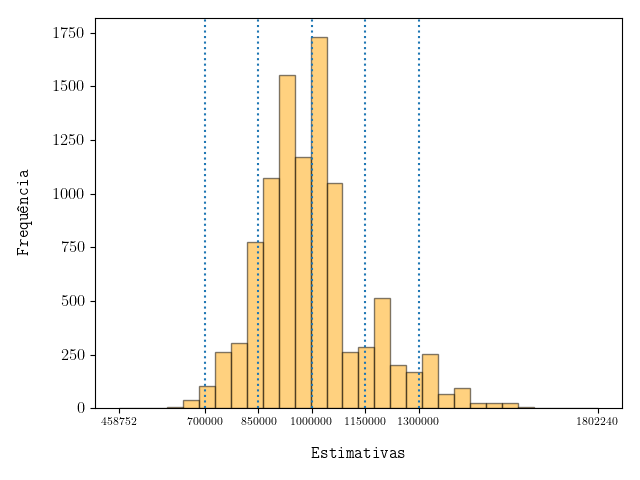
\includegraphics[width=\linewidth, height=4cm]{figuras/adaptive_sampling_variance_64.png}
    \label{fig:as:experimento:02:64}
  \end{subfigure}%
  \begin{subfigure}{.5\textwidth}
    \centering
    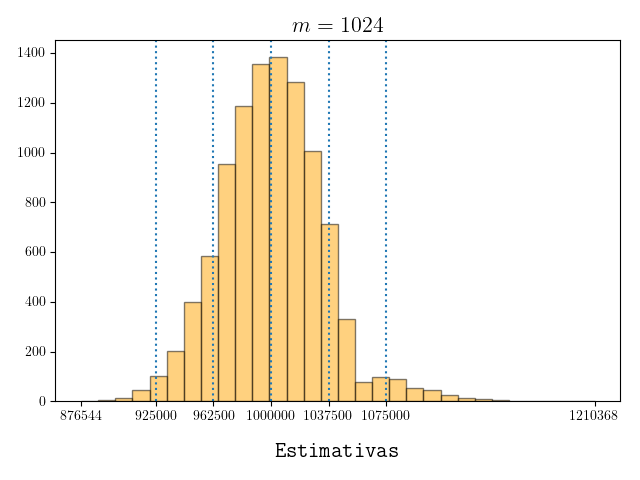
\includegraphics[width=\linewidth, height=4cm]{figuras/adaptive_sampling_variance_1024.png}
    \label{fig:as:experimento:02:1024}
  \end{subfigure}
  \caption{Segundo experimento do algoritmo $\AS$. Foram realizadas dez mil simulações e em cada simulação, foram 
    inseridos em estruturas~\texttt{AdaptiveSampling} com $m = 64$ e $m = 1024$, um milhão de inteiros de~64 bits 
    gerados uniformemente. Os resultados foram utilizados para a construção dos histogramas de frequência acima. }
  \label{fig:as:experimento:02}
\end{figure}

Com os experimentos apresentados nessa seção, foi possível termos noção da precisão do algoritmo das~$\asampling$. Este
algoritmo tem pontos interessantes, como se basear em padrões de bits para construir a estimativa e funcionar bem para
fluxos com poucos elementos. Porém, a principal desvantagem dessa solução é o consumo de memória. Se considerarmos uma
aplicação que precise lidar com hashes de 32~bits, então o consumo de memória da estrutura~\texttt{AdaptiveSampling} 
seria de pelos menos $32 \times m$~bits no pior caso, quando a lista $LIST$ passa a ter mais que $m$ elementos. Esse
custo é o mesmo que o do algoritmo~$\pcounting$, quando $L = 32$. Dessa forma, as $\asampling$, que tem um desvio maior
que a $\pcounting$, tem também um consumo de espaço pior. 

Para que esse gasto de memória fosse reduzido sem que se perdesse muita precisão, demorou mais de 20 anos desde a 
criação da $\pcounting$. Veremos na próxima seção como podemos reduzir ainda mais esse consumo.

\par

\chapter{\textbf{LogLog's}}

Em 1978, Morris resolveu o problema de estimar quantos elementos passaram por um fluxo de dados sem armazenar esse valor 
em um contador. E as ideias principais da \hyperref[chap:morris:algorithm]{solução dele} era guardar uma aproximação do 
logarítmo dessa quantidade e incrementá-la por meio de um método probabilístico que lembra lançamentos de moedas. Dessa 
forma, se temos um fluxo com $n$ elementos, e $X$ é a aproximação do algoritmo de Morris para~$\lg n$, então $X$ deve 
ser incrementado com probabilidade $1 \mathbin{/} 2^X$ para cada novo elemento, e isto é equivalente a lançarmos uma 
moeda $X$ vezes e aumentar $X$ somente se todas as jogadas forem cara. 

Essa solução inspirou o desenvolvimento do algoritmo da $\pcounting$, que resolvia o problema de estimar a quantidade de 
elementos distintos que passaram por um fluxo~$\Mbb$. Nesse \hyperref[sec:flajolet-martin:algorithm]{algoritmo}, estamos 
interessados em usar \hyperref[sec:flajolet-martin:pattern]{padrões de bits} de números inteiros aleatórios para gerar 
essa estimativa. Portanto, os dados de $\Mbb$ são mapeados para inteiros por meio de uma função de hash, e assim, 
podemos considerar que esses elementos são na verdade palavras binárias de tamanho infinito. Essa simplificação nos 
permite agrupar os itens de $\Mbb$ por prefixos da forma $0^{*}1$. A razão de fazermos isto é que a probabilidade de a 
representação binária de um inteiro ter um prefixo da forma $0^{X-1}1$ é $1 \mathbin{/} 2^{X}$, a mesma que aparece no 
algoritmo de Morris, e portanto, essa ideia pode ser usada para estimarmos o logarítmo da quantidade de elementos 
distintos em $\Mbb$ da seguinte forma: guardaremos o menor $R$ tal que ainda não tenha aparecido algum inteiro com 
prefixo~$0^{R}1$.

Dessa maneira, para um fluxo $\Mbb$ com $n$ elementos distintos, $R$ seria a estimativa para~$\lg n$. No entanto, por 
meio do cálculo do valor esperado desse estimador, é possível concluir que $R$, na verdade, não estima $\lg n$, mas 
$\lg \phi n$~\citep{flajolet:martin:85}. Em outras palavras, o algoritmo da $\pcounting$ produz uma estimativa com um 
desvio $\phi$ mensurável e podemos, em vista disso, corrigí-lo.

Contudo, mesmo corrigindo esse erro do estimador, este ainda possui uma grande variância, ou seja, a estimativa 
devolvida pode estar muito próxima ou muito longe do valor real. Para contornar essa situação, podemos repetir várias 
vezes o algoritmo da $\pcounting$ e encontrar a média dos estimadores. E uma forma interessante de se fazer isso em uma 
única iteração, removendo assim, a necessidade de executarmos o algoritmo muitas vezes, é dividir de modo uniforme os 
dados do fluxo em $m$ lotes. Então, um inteiro $x$ faria parte do lote $x \bmod m$, e olharíamos para o prefixo de 
$\lfloor x \mathbin{/} m \rfloor$. Desse modo, passaríamos a guardar um estimador $R$ para cada lote, e a estimativa 
para $n$ usaria a média desses valores. Essa técnica é conhecida como \textbf{média estocástica}.

Por fim, o algoritmo da $\pcounting$ tem consumo proporcional a $O(mL)$ bits, em que $m$ é o número de lotes e $L$ é a
quantidade de bits necessária para armazenar algum inteiro do fluxo. Esse consumo é decorrente do fato de cada lote 
precisar guardar a informação se um prefixo da forma $0^{*}1$ já apareceu, e podemos fazer isto com $L$ bits por lote. 
Nesse sentido, o próximo algoritmo, chamado $\LOG$, terá como base muitas ideias da $\pcounting$, e apresentará uma 
significativa redução do consumo de espaço.

\section{Algoritmo $\LOG$}
\label{sec:loglog:algorithm}

Dado um fluxo $\Mbb$ com $n$ elementos distintos, o algoritmo~$\LOG$ devolverá um estimador~$\hat{n}$ para $n$, que terá
um desvio padrão de $1{,}30 \mathbin{/} \sqrt{m}$~\citep{loglog:03}. Assim como foi feito no algoritmo da $\pcounting$, 
precisamos ter uma função de hash~$h$ que mapeie uniformemente os dados de um fluxo para inteiros. Tendo esta função em 
mãos, podemos supor que estamos trabalhando com um fluxo de inteiros aleatórios. E vamos manter o maior~$M$ tal que 
exista algum elemento em~$\Mbb$ cuja representação binária tenha prefixo da forma $0^{M-1}1$.

Para $M \geq 1$, a probabilidade de um inteiro ter um prefixo da forma~$0^{M-1}1$ é $1 \mathbin{/} 2^{M}$, ou seja, 
esperamos que um em cada $2^{M}$ elementos tenha esse prefixo. Por outro lado, podemos inverter essa ideia, e pensar que 
se temos um inteiro com prefixo da forma $0^{M-1}1$, então pelo menos $2^{M}$ elementos distintos devem ter aparecido. 
Desse modo, o valor de $M$ será uma aproximação para~$\lg n$, e podemos interpretá-lo como sendo a posição indexada a 
partir do 1 do bit ligado menos significativo de um inteiro. Uma ideia similar foi vista na 
Seção~\ref{sec:flajolet-martin:algorithm}, em que definimos a função $\rho$ que retorna a posição indexada a partir 0 do 
bit ligado menos significativo de um número. Em vista disso, vamos definir a função $\rho_1$ que retorna o valor 
anterior só que indexado a partir do 1, e utilizá-la para o cálculo de~$M$.

Para reduzirmos a variância da estimativa, dividimos o fluxo~$\Mbb$ em $m = 2^{k}$ lotes de acordo com os bits dos 
elementos. Dessa forma, um inteiro $x = \langle b_1 b_2 {\dots} b_k {\dots} \rangle$ fará parte do lote 
$y = \langle b_1 b_2 {\dots} b_k \rangle$, ou seja, os $k$ primeiros bits de um elemento indicam em qual lote ele 
pertence. Em seguida, encontramos $M_y$ tal que $0^{M_y}1$ é prefixo de $\langle b_{k+1} b_{k+2} {\dots} \rangle$, e 
mantemos o maior valor de $M_y$.

Desse modo, o valor de $M_y$ de cada lote~$y$ será uma estimativa para $\lg \frac{n}{m}$. Para diminuirmos a variância 
dessa aproximação, calculamos a média \textbf{aritmética} $\overline{M} = \frac{\sum_y M_y}{m}$. Logo, $\overline{M}$ 
aproxima $\lg \frac{n}{m}$, e consequentemente, $2^{\overline{M}}$ aproxima $\frac{n}{m}$. E, portanto, a estimativa 
para $n$ será $m \times 2^{\overline{M}}$.

No entanto, essa estimativa apresenta um desvio e para corrigí-lo, multiplicamos ela por uma constante $\alpha_m$ cujo 
valor é proporcional ao número de lotes utilizados no algoritmo. Na prática, podemos usar como fator de correção 
$\alpha_\infty \approx 0{,}39701$ assim que $m$ for maior que~64. Em vista disso, a saída do algoritmo~$\LOG$ será um 
estimador $\hat{n}$ da forma $\alpha_m \times m \times 2^{\overline{M}}$. E o pseudocódigo a seguir condensa as ideias 
apresentadas.

\begin{codebox}
  \Procname{$\logprogram\big(\Mbb, m = 2^k\big)$}
  \li \For $i$ de $0$ até $m$
        \Do
  \li   $M[i] \gets 0$
        \End
  \li \For cada $x$ em $\Mbb$ 
        \Do
  \li   $b_1b_2{\dots} \gets h(x)$
  \li   $lote \gets \langle b_1 {\dots} b_k \rangle$
  \li   $M[lote] \gets \max(M[lote], \rho_1(b_{k+1}b_{k+2}{\dots}))$
        \End
  \li
  \Return $\alpha_m \times m \times 2^{\frac{1}{m}\sum_i{M[i]}}$   
  \End
\end{codebox}

Vamos simular um exemplo pequeno para entendermos com mais detalhes o algoritmo~$\logprogram$. O objetivo, portanto, é 
estimar a quantidade de elementos distintos em $\Mbb = \{ 50, 85, 45, 29, 89, 82, 87, 10, 92 \}$. Suponhamos que 
$k = 2$, $m = 2^{k} = 2^2 = 4$, que a função de hash~$h$ seja a função identidade e que $\alpha_m = \alpha_4 = 1$, 
ou seja, estamos desconsiderando o desvio da estimativa devolvida pelo algoritmo. 

Inicialmente, os vetores $M$ estão zerados, ou seja, $M[i] = 0$ para $0 \leq i < 4$. Na primeira iteração do algoritmo,
temos que verificar em qual lote o elemento $50 = 010011_2$ se encontra. Como $k = 2$, os primeiros $2$ bits definem o
lote e assim, $50$ faz parte do lote $01_2 = 2$. Ao final da primeira iteração, temos que $M[2] = 3$, já que 
$\rho_1(0011_2) = 3$ e dessa forma, $0011_2$ tem prefixo da forma $0^21$

Na segunda iteração, o número do lote de $85 = 1010101_2$ é $1$, e $\rho_1(10101_2) = 1$. Desse modo, $M[1] = 1$. Os 
próximos elementos a serem considerados, $45 = 101101_2$ e $29 = 10111_2$, fazem parte do lote de número~$1$, e têm 
prefixo da forma $0^01$. Dessa maneira, $M[1]$ continua sendo um após esses itens serem processados. Precisamos, assim,
analisar $89 = 1001101_2$, que pertence ao lote~$1$. Como $\rho_1(01101_2) = 2$, $M[1]$ passa a ter valor $2$.

O próximo elemento de $\Mbb$ é $82 = 0100101_2$ cujo lote é $2$. Temos que $\rho_1(00101) = 3$, mas o valor de $M$ do 
lote~$2$ já é $3$, sendo assim, $M[2]$ continua com o mesmo valor. Continuando o exemplo, devemos processar 
$87 = 1110101_2$. Este item está no lote~$3$, e $\rho_1(10101_2) = 1$. Logo, $M[3]$ passa a ser igual a 1. No caso 
seguinte, $10 = 0101_2$ faz parte do lote $2$ e $\rho_1(01_2) = 2$. Contudo, $M[2]$ é maior que $2$ e portanto, não é 
atualizado. Por fim, $92 = 0011101_2$ vai para o lote~$0$, $\rho_1(11101_2) = 1$ e $M[0] = 1$.

Os valores de $M$ ao processarmos todos os elementos de $\Mbb$ são: $M[0] = 1$, $M[1] = 2$, $M[2] = 3$ e $M[3] = 1$. 
Logo, o valor médio $\overline{M}$ de $M$ é $(1 + 2 + 3 + 1) / 4 = 7 / 4 = 1{,}75$. E a estimativa para a quantidade de 
itens distintos em 
$\Mbb$ é $\alpha_m \times m \times 2^{\overline{M}} = 1 \times 4 \times 2^{1{,}75} = 13{,}45{\dots} \approx 13$.

\section{Consumo de espaço do $\LOG$}

No algoritmo da $\pcounting$, vimos a ideia de dividirmos os elementos de um fluxo de dados em $m$ lotes. E como cada 
lote armazena um vetor $\bitmap$ com $L$ bits, o consumo de espaço dessa solução é de $O(mL)$ bits. Assim, para 
$m = 1024$ e $L = 32$, a $\pcounting$ gasta $4$ KB de memória para estimar o número de itens distintos em um fluxo.

Por outro lado, o algoritmo~$\LOG$ também divide os dados de um fluxo $\Mbb$ com $n$ elementos distintos em $m$ lotes. 
Só que ao invés de um lote guardar a informação se um prefixo já apareceu ou não, ele armazena uma aproximação para 
$\lg n$. Logo, se para representarmos um inteiro~$x$, precisamos de pelo menos $\lg x$ bits, para guardar $\lg n$, são
necessários $\lg \lg n$ bits. Este fato deu origem ao nome do algoritmo.

Considerando o exemplo anterior em que $m = 1024 = 2^{10}$ e que os dados do fluxo são inteiros de $32$ bits, os 10 
primeiros bits definem o lote de um elemento e os 22 restantes serão utilizados para encontrar $M$. Dessa forma, temos 
que $M \leq 22$ e precisamos de somente $5$ bits para guardar esse valor. Portanto, o custo de espaço do 
algoritmo~$\LOG$ nesse caso é de $0{,}625$~KB, que é cerca de seis vezes menor que na $\pcounting$.

Essa diferença é maior ainda se trabalharmos com inteiros de $64$ bits e valores de $m$ na ordem de $65536 = 2^{16}$
para termos estimativas mais precisas. No algoritmo~$\LOG$, $M$ pode ser armazenado com 6 bits, pois $M \leq 48$, e 
desse modo, o custo de memória é de $50$~KB, dez vezes menos que na $\pcounting$, que gasta aproximadamente 
$524$~KB.

\section{Implementando $\LOG$}

\begin{lstlisting}[style=mypython,caption=Implementação do algoritmo $\logprogram$,captionpos=b, label=loglog:code]
class LogLog:
    def __init__(self, m=64):
        self.m = m
        self.B = math.floor(math.log2(m))
        self.M = [0] * m
        self.Z = 0
        self.alpha = 0.39701
  
    def p(self, x: int):
        return (x & -x).bit_length()

    @property
    def prefixo(self):
        return (1 << self.B) - 1

    def adiciona(self, x: int):
        lote = x & self.prefixo
        w = x >> self.B

        if self.p(w) > self.M[lote]:
            self.Z -= self.M[lote]
            self.M[lote] = self.p(w)
            self.Z += self.M[lote]

    def conta(self):
        Z_media = self.Z / self.m
        return math.floor(self.alpha * self.m * math.pow(2.0, Z_media))
\end{lstlisting}

A classe~\texttt{LogLog} do Programa~\ref{loglog:code} foi baseada no algoritmo~$\logprogram$. Vamos fazer alguns 
comentários sobre o método~\texttt{adiciona}. O primeiro deles é relacionado à identificação do lote de um elemento~$x$.
Nessa implementação, a variável \texttt{B} faz o papel da variável~$k$ do algoritmo~$\logprogram$. Vimos na 
Seção~\ref{sec:loglog:algorithm}, que os $k$ primeiros bits definem o lote. Logo, os \texttt{B} bits iniciais contém a
informação do lote de~$x$. Sabendo disto, precisamos de um modo de recortar esses bits. 

Um jeito de fazermos isto é montarmos um número tal que os primeiros \texttt{B} bits dele sejam~1 e os restantes, 0. 
Vamos chamá-lo de $y$. Nesse sentido, $x \mathbin{\&} y$ resultará em um inteiro $z$ cuja represetação binária tem as 
seguintes propriedades: os \texttt{B} primeiros bits correspondem aos \texttt{B} bits iniciais de $x$, e os bits 
restantes são zero. Portanto, $z$ é justamente o lote de~$x$. Falta, assim, saber como calcular $y$. Um número com as 
mesmas características de $y$ é~$2^{\texttt{B}} - 1$, e podemos calculá-lo usando o operador $<<$, que é equivalente à 
potenciação na base $2$ quando aplicado ao número~$1$.

Um exemplo que pode deixar a ideia anterior clara é o seguinte: suponha que $\texttt{B} = 2$. Logo, 
$2^{\texttt{B}} - 1 = 2^2 - 1 = 3 = 11_2$. Note que todos os bits de $3$ estão ligados até a posição~$2$. Tomemos alguns
valores para $x$, como $7 = 111_2$ e $13 = 1011_2$. O lote do elemento $7$ é 
$7 \mathbin{\&} 3 = 111_2 \mathbin{\&} 110_2 = 110_2 = 3$, e de 13, 
$13 \mathbin{\&} 3 = 1011_2 \mathbin{\&} 1100_2 = 1000_2 = 1$. Podemos ver que os lotes calculados batem de fato com os 
valores esperados.

Uma vez calculado o lote de um elemento~$x$, precisamos remover os \texttt{B} bits iniciais dele para que possamos 
prosseguir com o algoritmo. Um modo de fazermos isto é utilizando o operador $>>$ que remove os bits menos 
significativos de um inteiro. Assim, seja $w = x >> \texttt{B}$. A represetação binária de $w$ será a mesma que a de 
$x$, só que sem os primeiros \texttt{B} bits. Logo, tomando novamente $B = 2$ e $x = 13 = 1011_2$, $w$ seria igual a 
$1011_2 >> 2 = 11_2$.

Por fim, para que possamos ter um método \texttt{conta} com complexidade constante, precisamos ter a soma~$Z$ dos 
valores de $M$ já pré-computada para que a média deles seja calculada rapidamente. Dessa forma, a variável~$Z$ é mantida
atualizada a cada novo elemento inserido no método \texttt{adiciona}. 

\newpage
\section{Algoritmo $\HLOG$}
\label{sec:loglog:hyperloglog}

Apesar do algoritmo~$\LOG$ visto anteriormente ter um consumo de memória pelo menos $6$ menor que a $\pcounting$, o
desvio padrão dele, que é de $1{,}30 \mathbin{/} \sqrt{m}$, é maior. Isto pode ser um problema se tivermos que trabalhar 
com quantidades muito grandes, da ordem de bilhões. No entanto, com uma simples modificação no algoritmo~$\logprogram$, 
obtemos um novo algoritmo com o mesmo consumo de memória, mas desvio padrão de~$1{,}04 \mathbin{/} \sqrt{m}$.

O aprimoramento do algoritmo~$\LOG$ é conhecido como $\HLOG$~\citep{hyperloglog:07}. E a modificação que deve ser feita 
em~$\logprogram$ é substituir a média \textbf{aritmética} pela média \textbf{harmônica}. A intuição por trás desta 
substituição é que a média harmônica é afetada menos por \textit{outliers}, ou seja, valores muito fora do esperado não 
distorcem tanto a estimativa. A consequência disso é que a variância do estimador é reduzida. 

Tanto no algoritmo~$\LOG$ quanto no $\HLOG$, o valor de $M$ de cada lote é uma aproximação para $\lg n \mathbin{/} m$, e 
conseguimos obter uma estimativa para $n \mathbin{/} m$ se elevarmos~$2$ a esse valor. Dessa forma, no algoritmo~$\LOG$, 
a média aritmética das aproximações de $\lg n \mathbin{/} m$ é calculada. Por outro lado, no algoritmo~$\HLOG$, 
calculamos a média harmônica das aproximações de $n \mathbin{/} m$. Podemos encontrar esse média $\overline{M}$ da 
seguinte forma:

\[ \overline{M} = \bigg(\frac{\sum\big(2^{M[i]}\big)^{-1}}{m}\bigg)^{-1} = \frac{m}{\sum2^{-M[i]}} \]

O fato de trocarmos a média aritmética pela harmônica também interfere no fator de correção $\alpha_m$. Na prática, 
podemos usar a aproximação $\alpha_{\infty} \approx 0{,}7213$ assim que $m$ for maior que 128~\citep{HyperLogLogWiki}.
Por fim, o algoritmo~$\hlogprogram$ traduz essas ideias para pseudocódigo, e é possível notar que ele é praticamente 
idêntico ao algoritmo~$\logprogram$. A única diferença entre essas soluções está na última linha.

\begin{codebox}
      \Procname{$\hlogprogram(\Mbb, m = 2^k)$}
      \li \For $i$ de $0$ até $m$
            \Do
      \li   $M[i] \gets 0$
            \End
      \li \For cada $x$ em $\Mbb$ 
            \Do
      \li   $b_1b_2{\dots} \gets h(x)$
      \li   $lote \gets \langle b_1 {\dots} b_k \rangle$
      \li   $M[lote] \gets \max(M[lote], \rho_1(b_{k+1}b_{k+2}{\dots}))$
            \End
      \li
      \Return $\alpha_m \times m^2 \mathbin{/} \sum_i{2^{-M[i]}}$   
      \End
\end{codebox}

\newpage
\section{Implementando $\HLOG$}

\begin{lstlisting}[style=mypython,caption=Implementação do algoritmo $\hlogprogram$,captionpos=b, label=hloglog:code]
class HyperLogLog:
      def __init__(self, m=64):
          self.m = m
          self.B = math.floor(math.log2(m))
          self.M = [0] * m
          self.Z = self.m
          self.alpha = 0.7213
  
      def p(self, x: int):
          return (x & -x).bit_length()
  
      @property
      def prefixo(self):
          return (1 << self.B) - 1
  
      def adiciona(self, x: int):
          lote = x & self.prefixo
          w = x >> self.B
  
          if self.p(w) > self.M[lote]:
              self.Z -= math.pow(2, -self.M[lote])
              self.M[lote] = self.p(w)
              self.Z += math.pow(2, -self.M[lote])
  
      def conta(self):
          return math.floor(self.alpha * self.m * self.m / self.Z)
\end{lstlisting}

O Programa~\ref{hloglog:code} foi baseado no algoritmo~$\hlogprogram$ e é quase idêntico ao Programa~\ref{loglog:code}, 
que foi inspirado no algoritmo~$\logprogram$. Na implementação do $\LOG$, a variável~\texttt{Z} era a soma dos valores 
de \texttt{M}. Como no $\HLOG$, a média aritmética é substituída pela harmônica, a variável~\texttt{Z} passa a guardar 
outro tipo de soma. Em vista disso, o formato do estimador também muda, e consequentemente, o método~\texttt{conta} da 
classe \texttt{HyperLogLog} é ligeiramente diferente do mesmo método da classe \texttt{LogLog}.

Essa troca de médias também afeta o método~\texttt{adiciona}. As implementações apresentadas retornam a estimativa da 
quantidade de elementos distintos em tempo constante, e assim, a cada novo item inserido no método~\texttt{adiciona}, 
devemos atualizar a variável~\texttt{Z} para evitar computá-la toda vez que o método~\texttt{conta} for chamado. E é 
justamente essa atualização da variável~\texttt{Z} que difere nos dois programas.
\par